\documentclass[12pt,border=12pt]{standalone}
\usepackage[utf8]{inputenc}
\usepackage{tikz}
\usepackage{lmodern}
\usepackage{amsmath,amssymb}
\usetikzlibrary{arrows.meta,positioning,calc,fit,backgrounds,shadows}

\begin{document}
\fontsize{12pt}{15pt}\selectfont

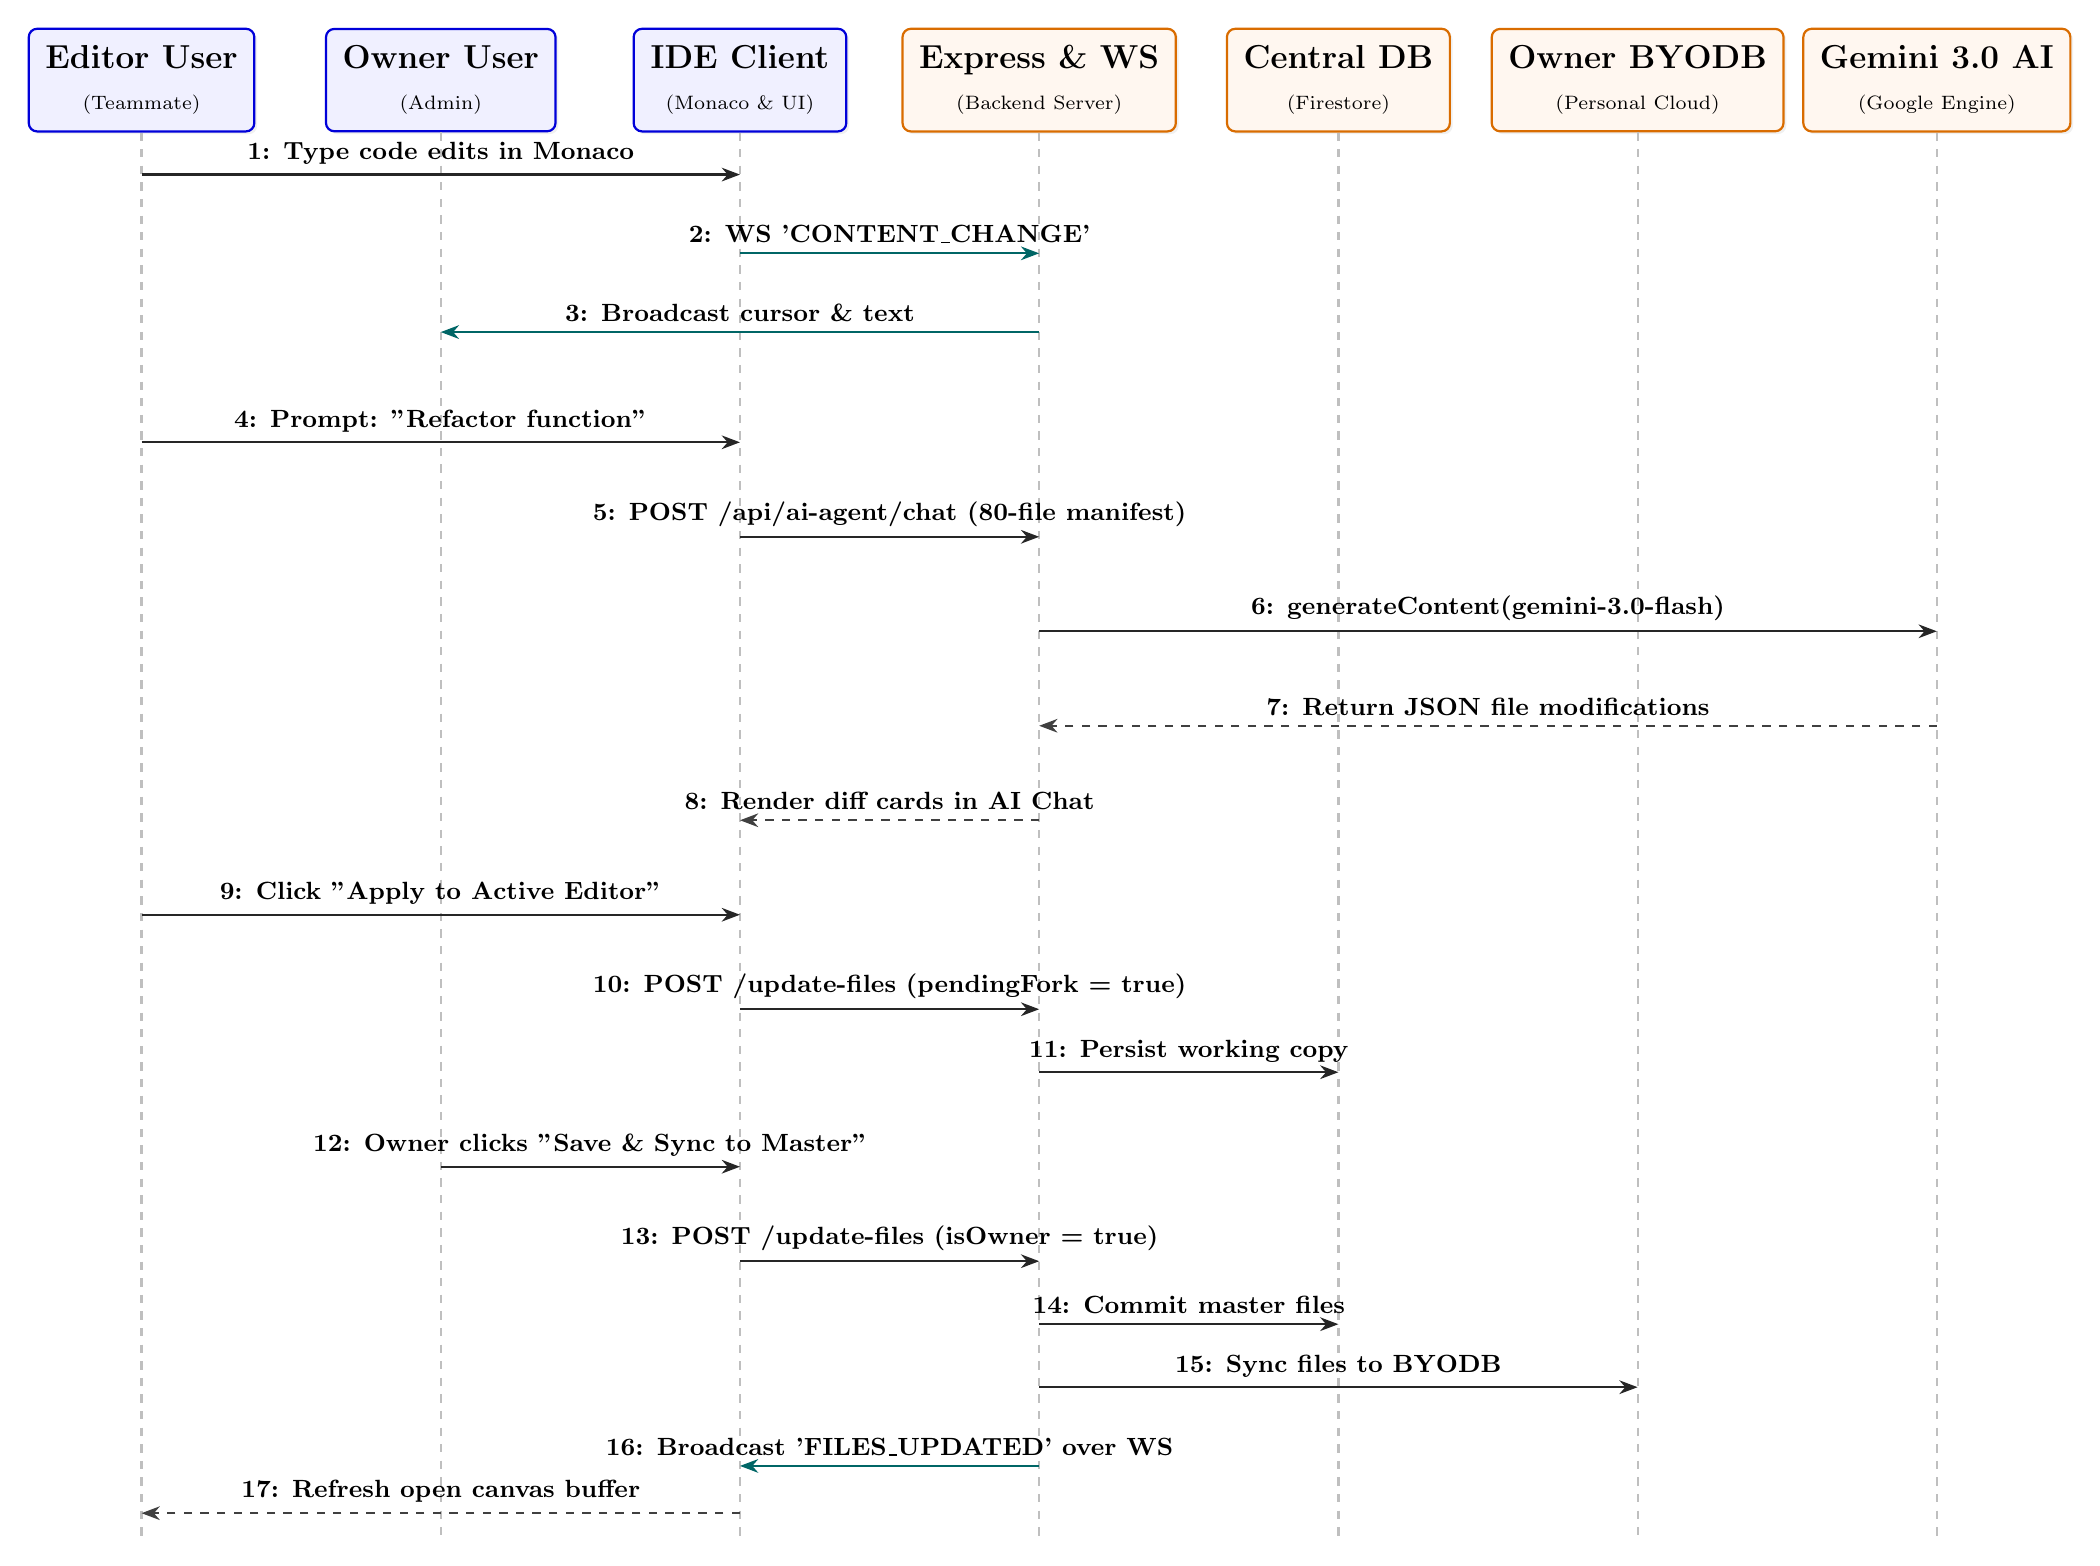
\begin{tikzpicture}[
    font=\fontsize{12pt}{15pt}\selectfont,
    >=Stealth,
    lifeline/.style={
        rectangle,
        draw=blue!85!black,
        fill=blue!6!white,
        thick,
        rounded corners=3pt,
        align=center,
        inner sep=6pt,
        minimum width=2.7cm,
        minimum height=1.1cm,
        drop shadow={opacity=0.12,shadow xshift=1pt,shadow yshift=-1pt}
    },
    systemLifeline/.style={
        rectangle,
        draw=orange!85!black,
        fill=orange!6!white,
        thick,
        rounded corners=3pt,
        align=center,
        inner sep=6pt,
        minimum width=2.7cm,
        minimum height=1.1cm,
        drop shadow={opacity=0.12,shadow xshift=1pt,shadow yshift=-1pt}
    },
    lineDash/.style={
        draw=gray!50,
        dashed,
        thick
    },
    syncMsg/.style={
        thick,
        draw=black!85,
        ->
    },
    asyncMsg/.style={
        thick,
        draw=teal!80!black,
        ->
    },
    replyMsg/.style={
        thick,
        dashed,
        draw=black!75,
        ->
    },
    noteBox/.style={
        rectangle,
        draw=yellow!80!black,
        fill=yellow!10!white,
        rounded corners=3pt,
        inner sep=4pt,
        font=\fontsize{10.5pt}{12pt}\selectfont
    }
]

% ==================== LIFELINE HEADERS ====================
\node[lifeline] (edUser) at (0, 0) {\textbf{Editor User}\\\scriptsize (Teammate)};
\node[lifeline] (ownUser) at (3.8, 0) {\textbf{Owner User}\\\scriptsize (Admin)};
\node[lifeline] (ideClient) at (7.6, 0) {\textbf{IDE Client}\\\scriptsize (Monaco \& UI)};
\node[systemLifeline] (collabServer) at (11.4, 0) {\textbf{Express \& WS}\\\scriptsize (Backend Server)};
\node[systemLifeline] (centralDB) at (15.2, 0) {\textbf{Central DB}\\\scriptsize (Firestore)};
\node[systemLifeline] (byodb) at (19.0, 0) {\textbf{Owner BYODB}\\\scriptsize (Personal Cloud)};
\node[systemLifeline] (geminiAI) at (22.8, 0) {\textbf{Gemini 3.0 AI}\\\scriptsize (Google Engine)};

% Vertical Lifeline Rails
\def\seqEnd{-18.5}
\draw[lineDash] (edUser.south) -- (0, \seqEnd);
\draw[lineDash] (ownUser.south) -- (3.8, \seqEnd);
\draw[lineDash] (ideClient.south) -- (7.6, \seqEnd);
\draw[lineDash] (collabServer.south) -- (11.4, \seqEnd);
\draw[lineDash] (centralDB.south) -- (15.2, \seqEnd);
\draw[lineDash] (byodb.south) -- (19.0, \seqEnd);
\draw[lineDash] (geminiAI.south) -- (22.8, \seqEnd);

% ==================== INTERACTIONS ====================

% 1. Code Edit
\draw[syncMsg] (0, -1.2) -- node[above, font=\small\bfseries] {1: Type code edits in Monaco} (7.6, -1.2);

% 2. WS Broadcast Content
\draw[asyncMsg] (7.6, -2.2) -- node[above, font=\small\bfseries] {2: WS 'CONTENT\_CHANGE'} (11.4, -2.2);

% 3. Peer Broadcast
\draw[asyncMsg] (11.4, -3.2) -- node[above, font=\small\bfseries] {3: Broadcast cursor \& text} (3.8, -3.2);

% 4. AI Prompting
\draw[syncMsg] (0, -4.6) -- node[above, font=\small\bfseries] {4: Prompt: "Refactor function"} (7.6, -4.6);

% 5. Send to AI Backend
\draw[syncMsg] (7.6, -5.8) -- node[above, font=\small\bfseries] {5: POST /api/ai-agent/chat (80-file manifest)} (11.4, -5.8);

% 6. Invoke Gemini API
\draw[syncMsg] (11.4, -7.0) -- node[above, font=\small\bfseries] {6: generateContent(gemini-3.0-flash)} (22.8, -7.0);

% 7. Return Code Modifications
\draw[replyMsg] (22.8, -8.2) -- node[above, font=\small\bfseries] {7: Return JSON file modifications} (11.4, -8.2);

% 8. Render Modification Cards
\draw[replyMsg] (11.4, -9.4) -- node[above, font=\small\bfseries] {8: Render diff cards in AI Chat} (7.6, -9.4);

% 9. Apply Patch to Working Copy
\draw[syncMsg] (0, -10.6) -- node[above, font=\small\bfseries] {9: Click "Apply to Active Editor"} (7.6, -10.6);

% 10. Save Working Copy (pendingFork)
\draw[syncMsg] (7.6, -11.8) -- node[above, font=\small\bfseries] {10: POST /update-files (pendingFork = true)} (11.4, -11.8);
\draw[syncMsg] (11.4, -12.6) -- node[above, font=\small\bfseries] {11: Persist working copy} (15.2, -12.6);

% 11. Owner Reviews & Syncs Master
\draw[syncMsg] (3.8, -13.8) -- node[above, font=\small\bfseries] {12: Owner clicks "Save \& Sync to Master"} (7.6, -13.8);

% 12. Master Commit & Personal BYODB Sync
\draw[syncMsg] (7.6, -15.0) -- node[above, font=\small\bfseries] {13: POST /update-files (isOwner = true)} (11.4, -15.0);
\draw[syncMsg] (11.4, -15.8) -- node[above, font=\small\bfseries] {14: Commit master files} (15.2, -15.8);
\draw[syncMsg] (11.4, -16.6) -- node[above, font=\small\bfseries] {15: Sync files to BYODB} (19.0, -16.6);

% 13. Instant Peer Canvas Refresh
\draw[asyncMsg] (11.4, -17.6) -- node[above, font=\small\bfseries] {16: Broadcast 'FILES\_UPDATED' over WS} (7.6, -17.6);
\draw[replyMsg] (7.6, -18.2) -- node[above, font=\small\bfseries] {17: Refresh open canvas buffer} (0, -18.2);

\end{tikzpicture}
\end{document}
